\documentclass{article}
\usepackage{amsmath,amssymb,amsthm}
\usepackage{graphicx} % Required for inserting images
\usepackage{multicol}
\usepackage[letterpaper]{geometry}
\usepackage[colorlinks]{hyperref}

\title{Algebra 1 Practice Problems II}
\author{Alan Zhou}
\date{2023 - 2024}

\setlength{\parindent}{0pt}
\setlength{\parskip}{3pt plus 1pt minus 1pt}



\begin{document}

\maketitle

\section{Graphing}

\begin{enumerate}
\item Draw a coordinate plane and label the origin and the four quadrants.
\item Let $A = (3,1)$. Find the coordinates of each of the following:
\begin{enumerate}
\item the reflection of $A$ across the $x$-axis
\item the rotation of $A$ around the origin by $180^{\circ}$
\item the rotation of $A$ around the origin by $90^{\circ}$ counterclockwise
\item the reflection of $A$ across the $y$-axis
\item the reflection of $A$ across the line $y = x$
\item the rotation of $A$ around the point $(2,2)$ by $90^{\circ}$ clockwise
\end{enumerate}
\item The points $(5,7)$ and $(8,-1)$ lie on the line with equation $y = mx + b$, where $m$ and $b$ are constants. Find $m$ and $b$.
\item Which of the following expressions correctly finds the slope between the points $(-1,7)$ and $(3,-4)$? Circle all that apply.
% write some expressions here
\item Let $A = (1,1)$, $B = (5,2)$, and $C = (-4,3)$. In this problem, we will find the coordinates of the point $D$ for which quadrilateral $ABCD$ is a parallelogram.
\begin{enumerate}
\item Find the slopes of lines $AB$ and $BC$.
\item Write down an equation for the line through $C$ parallel to $AB$.
\item Write down an equation for the line through $A$ parallel to $BC$.
\item Since $AB\parallel CD$ and $AD\parallel BC$, point $D$ must be the intersection of the lines you found in parts (b) and (c). Use this to find the coordinates of point $D$.
\end{enumerate}
\item \begin{enumerate}
\item Of the equations
\begin{equation*}
5x + 4y = 35;\quad (x + 4)^2 + (y - 1)^2 = 10;\quad x^2 + xy + y^2 = 49;\quad x - 2y = -7,
\end{equation*}
which one is an equation for the blue line below?
\item Of the equations
\begin{equation*}
5x + 4y = 35;\quad (x + 4)^2 + (y - 1)^2 = 10;\quad x^2 + xy + y^2 = 49;\quad x - 2y = -7,
\end{equation*}
which one is an equation for the red curve below?
\end{enumerate}
\begin{center}
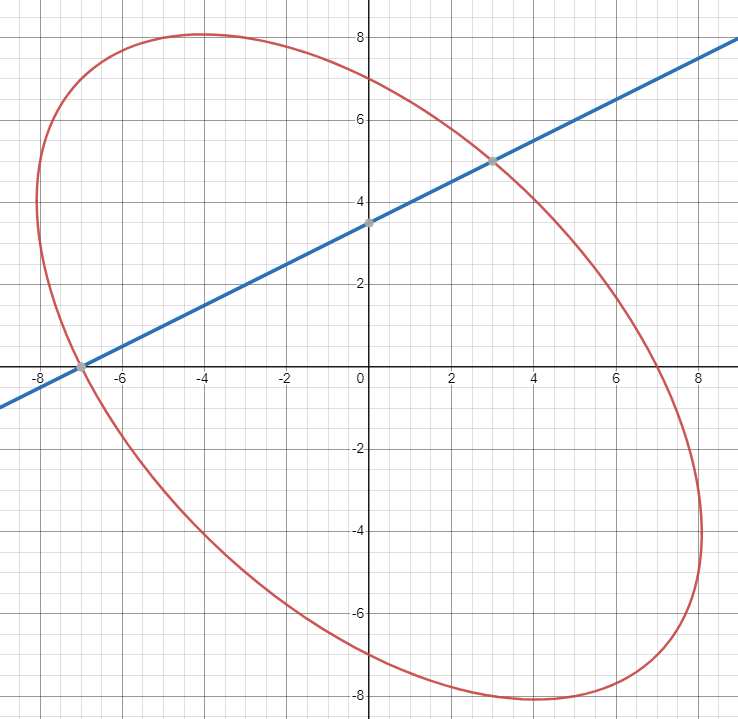
\includegraphics[scale=0.5]{03.png}
\end{center}
\end{enumerate}



% \item Draw graphs for each of the following equations:
% \begin{enumerate}
% \item $2x + 3y = 6$
% \item $y = (1/2)x + 3$
% \item $x = -y - 1$
% \item $y = \lvert x\rvert$
% \item $x = y^2 + 2$
% \item (Challenge) $y^2 = x(x + 1)(x - 1)$
% \end{enumerate}
% \item \begin{enumerate}
% \item When solving a system of two equations for variables $x$ and $y$, Polly finds that the graphs of the equations are parallel lines. How many solutions are there to the system?
% \item For another system, Quaresma finds that the graphs of the equations are the same line. How many solutions are there to this second system?
% \end{enumerate}
% \item What are the slope and the intercepts of the line given by the equation $4x - 7y = 84$?
% \item Let $O = (0,0)$, $P = (14,0)$, and $Q = (5,12)$.
% \begin{enumerate}
% \item What are the side lengths of triangle $OPQ$?
% \item What are the slopes of the sides of triangle $OPQ$?
% \end{enumerate}
% \item (Centroid) Let $A = (5,1)$, $B = (-1,3)$, and $C = (3,7)$.
% \begin{enumerate}
% \item Suppose $D$, $E$, and $F$ are the midpoints of $\overline{BC}$, $\overline{CA}$, and $\overline{AB}$, respectively. What are the coordinates of $D$, $E$, and $F$?
% \item Write down equations for lines $\overleftrightarrow{AD}$, $\overleftrightarrow{BE}$, and $\overleftrightarrow{CF}$.
% \item These three lines intersect at a single point (draw them!), called the \emph{centroid} of triangle $ABC$. What are the coordinates of the centroid?
% \end{enumerate}
% \item Let $A = (0,2)$ and $B = (12,8)$.
% \begin{enumerate}
% \item Let $P = (x,y)$. Write down expressions for $(AP)^2$ and $(BP)^2$.
% \item If $AP = BP$, then $P$ must lie on a certain line. What are the slope and $y$-intercept of that line?
% \item Where does that line intersect $\overline{AB}$?
% \end{enumerate}
% \end{enumerate}

% \newpage
% \section{Answers}

% \begin{multicols}{2}
% \begin{enumerate}
% \item \begin{enumerate}
% \item $n = 16$
% \item $4$
% \item $472$
% \item greater than 0
% \item greater than 1
% \item $-2$
% \item $4$
% \item $\dfrac{b^3c^9}{8a^6}$
% \end{enumerate}
% \item \begin{enumerate}
% \item 10
% \item $2\sqrt{2}$
% \item $6\sqrt{6}$
% \item $17\sqrt{7}$
% \item $2\sqrt[3]{18}$
% \item $3\sqrt{3}$
% \item $14\sqrt{2}$
% \item $\dfrac{2\sqrt{3542}}{119}$
% \end{enumerate}
% \item $x = 1$
% \item \begin{enumerate}
% \item $6x^2y + 7xy^2$
% \item $15a^3b^2 - 5a^3b^3$
% \item $-6x + 12x^2 + 18x^3$
% \item $-4a - 3b + 2ab$
% \end{enumerate}
% \item \begin{enumerate}
% \item $a^2 + 2ab + b^2$
% \item $a^2 - 2ab + b^2$
% \item $a^2 - b^2$
% \end{enumerate}
% \item \begin{enumerate}
% \item $2x(x - 9)$
% \item $xy(6x + 7y)$
% \item $9b(-7a^2 - 6ab + 5a + 4)$
% \item $(a - b)(a + b)$
% \item $(u - v)^2$ or $(v - u)^2$
% \item $(p + q)^2$
% \end{enumerate}
% \item \begin{enumerate}
% \item $\dfrac{x^3 + x^2 + x - 1}{x^2}$
% \item $\dfrac{x^2 + y^2}{xy}$
% \item $\dfrac{xy^2}{3}$
% \item $\dfrac{a}{a + b}$
% \end{enumerate}
% \item $m^2 + 4mn + 4n^2$
% \item $(a^2 + 2b^2 - 2ab)(a^2 + 2b^2 + 2ab)$
% \item \begin{enumerate}
% \item $x = 2$
% \item $a = 8/3$
% \item no solution
% \item all real numbers
% \end{enumerate}
% \item \begin{enumerate}
% \item $x = 5 - 7y$
% \item $y = \dfrac{5 - x}{7}$
% \item $b = \dfrac{-ax^2 - c}{x}$
% \item $p = \dfrac{-qr + q + r + 1}{qr + q + r - 1}$
% \end{enumerate}
% \item \begin{enumerate}
% \item $(x,y) = (1,1)$
% \item no solution
% \item $(x,y) = (-1,2)$
% \item all pairs $(x,y)$ such that $7x - 5y = 1$
% \item $(x,y) = (3,4)$
% \end{enumerate}
% The system has a unique solution if and only if $AD - BC\neq 0$.
% \item 20
% \item \begin{enumerate}
% \item \$132 (Add up all of the purchases)
% \item Pencils are \$0.50, binders are \$1.50, calculators are \$130
% \end{enumerate}
% \item \begin{enumerate}
% \item $7$
% \item $18$
% \item $52$
% \item $91$
% \item $19$
% \item $2$
% \item $399$
% \end{enumerate}
% \item \begin{enumerate}
% \item $N/F = 5/4$
% \item $340$
% \end{enumerate}
% \item $49/3$ tsp soy sauce, $35/3$ tsp sesame oil
% \item \begin{enumerate}
% \item $187\,500$ miles per second
% \item $\approx 186\,012$ miles per second
% \end{enumerate}
% \item \begin{enumerate}
% \item $1/6$
% \item $504$
% \end{enumerate}
% \item After one hour, $1/3$ of the pool is full. For the second hour, the pool fills at a rate of $(1/3) - (1/2) = -1/6$ of the pool per hour, so after the second hour, $1/6$ of the pool is full. Afterwards, the fill rate is $(1/3) + (1/4) - (1/2) = 1/12$ of the pool per hour, and we have $5/6$ of the pool left, so the answer is $(5/6) / (1/12) = \boxed{10}$ hours.
% \item Let $F$ be the time spent at $60$ miles per hour and $S$ be the time spent at $41$ miles per hour. The total time for the trip was $450 / 45 = 10$ hours, so $F + S = 3$. Also, we need $60F + 41S = 142$. Solving yields $F = 1$ and $S = \boxed{2}$ hours.
% \item \begin{enumerate}
% \item This can happen when a much higher proportion of Hospital Y's operations are type A (lower risk) compared to Hospital X. Given these numbers, only 50\% of Hospital X's operations are type A, vs 80\% of Hospital Y's.
% \item Hospital X
% \end{enumerate}
% \item \begin{enumerate}
% \item $\$144$
% \item $\$112$
% \item On January 1, 2001, the balance is $1.2(100 - X) = 120 - 1.2X$. Then, on January 1, 2002, the balance is $1.2(120 - 1.2X - X) = 144 - 2.64X$. This is paid off in full by the last $X$, so $144 - 2.64X = X$, so $X\approx\boxed{39.56}$.
% \end{enumerate}
% \item $75$
% \item See \href{https://www.desmos.com/}{Desmos}
% \item \begin{enumerate}
% \item none
% \item infinitely many
% \end{enumerate}
% \item Slope $4/7$\par $x$-intercept $(21,0)$\par $y$-intercept $(0,-12)$
% \item \begin{enumerate}
% \item $OP = 14$, $PQ = 15$, $QO = 13$
% \item $\overline{OP}$ has slope 0\par $\overline{PQ}$ has slope $-4/3$\par $\overline{QO}$ has slope $12/5$
% \end{enumerate}
% \item \begin{enumerate}
% \item $D = (1,5)$\par $E = (4,4)$\par $F = (2,2)$
% \item $\overleftrightarrow{AD}$ is $y = -x + 6$\par $\overleftrightarrow{BE}$ is $y - 3 = (1/5)(x + 1)$\par $\overleftrightarrow{CF}$ is $y = 5x - 8$
% \item $(7/3, 11/3)$
% \end{enumerate}
% \item \begin{enumerate}
% \item $(AP)^2 = x^2 + (y - 2)^2$\par $(BP)^2 = (x - 12)^2 + (y - 8)^2$
% \item Expand $(AP)^2 = (BP)^2$ and cancel squares: $-4y + 4 = -24x - 16y + 208$. This means $12y = -24x + 204$, so $y = -2x + 17$. The slope is $\boxed{-2}$ and the $y$-intercept is $\boxed{(0,17)}$.
% \item $(6,5)$  (This is the midpoint of $\overline{AB}$.)
% \end{enumerate}
% \end{enumerate}
% \end{multicols}


\end{document}
